\documentclass{article}
\usepackage{tikz}
\usetikzlibrary{positioning}

\begin{document}

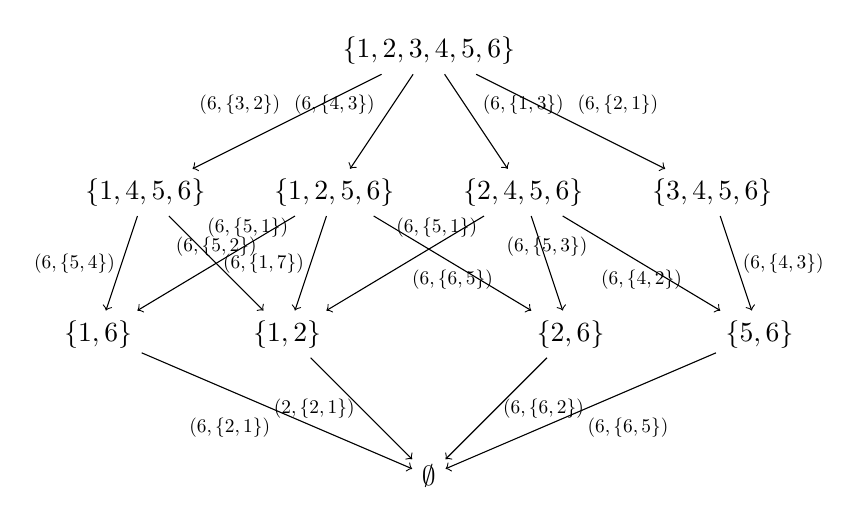
\begin{tikzpicture}[scale=1.2]
    % Define the vertices
    % Top level
    \node (top) at (0,5) {$\{1,2,3,4,5,6\}$};
    
    % Second level
    \node (n145) at (-3,3.5) {$\{1,4,5,6\}$};
    \node (n125) at (-1,3.5) {$\{1,2,5,6\}$};
    \node (n245) at (1,3.5) {$\{2,4,5,6\}$};
    \node (n345) at (3,3.5) {$\{3,4,5,6\}$};
    
    % Third level
    \node (n16) at (-3.5,2) {$\{1,6\}$};
    \node (n12) at (-1.5,2) {$\{1,2\}$};
    \node (n26) at (1.5,2) {$\{2,6\}$};
    \node (n56) at (3.5,2) {$\{5,6\}$};
    
    % Bottom level
    \node (empty) at (0,0.5) {$\emptyset$};
    
    % Define the edges
    % From top to second level
    \draw[->] (top) -- node[above left, scale=0.7] {$(6,\{3,2\})$} (n145);
    \draw[->] (top) -- node[above left, scale=0.7] {$(6,\{4,3\})$} (n125);
    \draw[->] (top) -- node[above right, scale=0.7] {$(6,\{1,3\})$} (n245);
    \draw[->] (top) -- node[above right, scale=0.7] {$(6,\{2,1\})$} (n345);
    
    % From second level to third level
    \draw[->] (n145) -- node[left, scale=0.7] {$(6,\{5,4\})$} (n16);
    \draw[->] (n145) -- node[above, scale=0.7] {$(6,\{5,2\})$} (n12);
    \draw[->] (n125) -- node[left, scale=0.7] {$(6,\{1,7\})$} (n12);
    \draw[->] (n125) -- node[below, scale=0.7] {$(6,\{6,5\})$} (n26);
    \draw[->] (n245) -- node[above, scale=0.7] {$(6,\{5,3\})$} (n26);
    \draw[->] (n245) -- node[below, scale=0.7] {$(6,\{4,2\})$} (n56);
    \draw[->] (n345) -- node[right, scale=0.7] {$(6,\{4,3\})$} (n56);
    
    % From third level to bottom
    \draw[->] (n16) -- node[below left, scale=0.7] {$(6,\{2,1\})$} (empty);
    \draw[->] (n12) -- node[left, scale=0.7] {$(2,\{2,1\})$} (empty);
    \draw[->] (n26) -- node[right, scale=0.7] {$(6,\{6,2\})$} (empty);
    \draw[->] (n56) -- node[below right, scale=0.7] {$(6,\{6,5\})$} (empty);
    
    % Additional edges (crossing edges)
    \draw[->] (n125) -- node[pos=0.3, above, scale=0.7] {$(6,\{5,1\})$} (n16);
    \draw[->] (n245) -- node[pos=0.3, above, scale=0.7] {$(6,\{5,1\})$} (n12);
    
\end{tikzpicture}

\end{document}